\documentclass[10pt,a4paper]{article}

\usepackage[margin=1in]{geometry}
\usepackage[T1]{fontenc}
\usepackage{amsmath,amssymb,amsthm}
\usepackage{graphicx}
\usepackage{booktabs}
\usepackage{tabularx}
\usepackage{array}
\usepackage{xcolor}
\usepackage{xurl}
\usepackage[numbers,sort&compress]{natbib}
\usepackage{hyperref}
\usepackage{enumitem}
\usepackage{caption}

\hypersetup{colorlinks=true, linkcolor=blue!50!black, citecolor=blue!50!black,
            urlcolor=blue!50!black}
\captionsetup{font=small, labelfont=bf}
\setlist{nosep, leftmargin=1.4em}
\sloppy
\emergencystretch=3em

\newtheorem{proposition}{Proposition}
\theoremstyle{definition}
\newtheorem{definition}{Definition}
\theoremstyle{remark}
\newtheorem{remark}{Remark}

\newcommand{\FF}{\mathbb{F}}
\newcommand{\ZZ}{\mathbb{Z}}
\newcommand{\Fb}{\mathcal{F}}
\newcommand{\abs}[1]{\lvert #1 \rvert}
% A committed artefact in this repository (or a sibling, with its prefix).
\newcommand{\art}[1]{\path{#1}}
\newcommand{\cls}[1]{\textsc{#1}}

\title{Ratcheting Elliptic-Curve Index Calculus Toward Pollard Rho:\\[4pt]
       {\large A Ledger of Verified Improvements, the Distance That Remains,\\
       and the Claims That Did Not Survive (July--October 2026)}}
\author{Anonymous}
\date{23 October 2026}

\begin{document}
\maketitle

\begin{abstract}
Pollard rho remains the fastest known algorithm for the discrete logarithm on
a prime-order elliptic curve. Index calculus, which can in principle exploit
more structure, has never beaten it on curves of cryptographic shape. Between
July and October 2026 we treated closing that gap as a \emph{ratchet}. Each
verified, measured improvement over the current best index-calculus pipeline
became the new baseline, and every row reports its remaining distance to a
matched rho. This paper is the ledger of that work, written from committed
evidence and current to 23 October 2026.

We organise the improvements by the stage they act on.
\begin{itemize}
\item \emph{Decomposition oracle.} Root-finding and meet-in-the-middle
  oracles are $383$--$1{,}535\times$ cheaper per decomposition than matrix
  F4, and up to $10^5\times$ cheaper than the earlier point-decomposition
  oracle. Inherited F4 does $199$--$222\times$ less matrix work than matrix
  F4. An $\FF_p$ F4 reaches msolve parity. A gate-first order and a
  root-rank harvest gate each cut the Gr\"obner work further, by
  $1.3$--$1.7\times$ and $1.41\times$.
\item \emph{Factor base and relation yield.} Free relations ($0.960\times$),
  re-randomised targets ($0.531\times$), a greedy coverage base, and a
  confirmed $n=83$ base selection ($1.195$\,s of $115$\,s cold).
\item \emph{Set-up and linear algebra.} A stacked $n=83$ producer
  ($3.24\times$ cold), a cache-blocked pair table ($0.24\times$ set-up), and
  CADO-style sparse linear algebra ($10.4\times$).
\item \emph{Two families whose fitted cost exponent lies below rho's.}
  Genus-three index calculus after the cubic GHS transfer, whose whole solve
  moved from $q^{1.91}$ to a local $q^{1.36}$ over five rounds. Gaudry's
  $k=4$ index calculus with FGHR's $D_4$ symmetry, $370$--$481\times$
  cheaper per decomposition, whose gap to rho closes as $n^{-1/4}$ from
  $5{,}080\times$ to $6.1\times$.
\end{itemize}

The distance remaining is stated plainly. On Koblitz curves of 36.6--47.2
bits, against a matched rho, the cold gap is $4.67$--$18.07\times$. On prime
curves it is $10.5\times$ at 20 bits and grows to $102\times$ at 40. The
nearest families are genus three ($1.15\times$ a measured rho at $q=2^{20}$)
and $k=4$ in characteristic two ($4.3\times$ a measured rho at $n\approx2^{56}$,
one target). Neither is a deployed curve shape.

We also report the claims that did not survive. All online wins over rho are
retired: Bernstein--Lange preprocessing rho with equal advice is
$53$--$317\times$ faster. Pricing native work and matching the rho reference
each raised a recorded gap, and a replay regression was traced to a
cross-ISA counter divergence. As of
this writing no index-calculus leaderboard row has passed the repository's
validation gate. Nothing here is a speed-up on a deployed curve or a key
recovery.

\end{abstract}

\tableofcontents
\bigskip

\section{Introduction}\label{sec:intro}

Let $\langle G\rangle$ be a subgroup of prime order $r$ of an elliptic
curve $E/\FF_q$. The best generic algorithm for its discrete-logarithm
problem is Pollard rho~\cite{pollard1978,vanoorschot1999}. When $A$
efficiently computable automorphisms act on the subgroup, rho costs about
$\sqrt{\pi r/(2A)}$ group additions~\cite{wiener1998,gallant2000}. Index
calculus was brought to elliptic curves through Semaev's summation
polynomials~\cite{semaev2004} and the extension-field analyses of Gaudry and
Diem~\cite{gaudry2009,diem2011}. It is the method that should exploit the
most structure. On prime-order curves of cryptographic shape it has never
beaten rho.

This paper does not ask whether index calculus beats rho; at every size we
can measure, it does not. It records how far a sustained engineering
programme moved index calculus \emph{toward} rho, one verified step at a
time, and how far remains.

\paragraph{The success criterion.} On 15 October 2026 the repository's owner
fixed the rule that governs this paper (\art{AGENTS.md}, ``Success
criterion: iterative improvement of the index-calculus baseline''):
\begin{itemize}
\item the baseline for each curve and size is the best current verified
  index-calculus pipeline, frozen with its protocol and receipts;
\item an \emph{improvement} lowers cost against that baseline on the same
  instances, with every answer verified, under a protocol frozen before
  timing;
\item each landed improvement becomes the new baseline (the ratchet);
\item every row reports its gap to the matched rho as the distance
  remaining, not as a pass/fail gate;
\item relabelling and accounting changes are recorded but are not
  improvements.
\end{itemize}
Beating rho remains the long-term goal, and a claim to have done so still
needs a cold, end-to-end, independently replayed win at growing sizes. No
such claim appears here.

\paragraph{Relation to the programme record.} A companion record
(\cite{icprogram2026}, \art{papers/ecdlp-index-calculus-program/}) surveys
the literature, the measurement infrastructure and the programme's
chronology through 20 October. This paper takes a narrower view in three
ways:
\begin{enumerate}
\item it organises the work by the pipeline stage each change acts on
  (\S\S\ref{sec:oracle}--\ref{sec:families}), and states each change
  against its own incumbent;
\item it collects the distance to rho by curve family, as it stands after
  the 19--20 October corrections, including the matched-rho re-run of the
  Koblitz rule (\S\ref{sec:distance});
\item it adds the work of 20--23 October: the confirmed $n=83$ base
  selection, the cache-blocked pair table, the planner validation, the
  ECCp-131 relation probes, the cross-ISA root cause of the replay
  regression, and the state of the validation gate
  (\S\S\ref{sec:audit}--\ref{sec:gate}).
\end{enumerate}
Where the two papers overlap, this one cites the same committed artefacts.
It ran no new measurement.

\paragraph{Contributions.}
\begin{itemize}
\item A cost decomposition of elliptic-curve index calculus into the levers
  the programme actually pulled, and the share of total cost each one
  controls (\S\ref{sec:model}).
\item The ratchet: about thirty improvements, each against its own
  incumbent, with boundary, class, interval and source
  (Figure~\ref{fig:ratchet}, Table~\ref{tab:ledger}).
\item The distance to matched rho, by family and size, with the reference
  each figure uses (\S\ref{sec:distance}).
\item An audit trail of claims that were corrected, and why each correction
  moved the gap \emph{up} (\S\ref{sec:audit}).
\item The state of the validation gate and what each row needs to pass it
  (\S\ref{sec:gate}).
\item The next improvements, ranked by the stage that now dominates cost
  (\S\ref{sec:next}).
\end{itemize}

\paragraph{What this paper does not claim.}
\begin{itemize}
\item No ECDLP speed-up on any deployed curve, and no key recovery.
\item No asymptotic sub-rho algorithm for prime fields, and no change to
  the Gaudry--Diem picture.
\item No statement about ECC2K-130, P-256 or secp256k1 security.
\end{itemize}
Every instance is a public synthetic or standard-parameter known-answer
instance. Stage ratios are never presented as end-to-end speed-ups. Wall
times from hosts without a qualifying isolation level are labelled
\emph{descriptive}. A cost with unpriced work is labelled a \emph{lower
bound}.

\paragraph{Reading the numbers.} We use two conventions.
\begin{itemize}
\item In the ledger (\S\S\ref{sec:oracle}--\ref{sec:families}) a ratio is
  \emph{candidate/incumbent}, so less than 1 is an improvement. Where a
  source reports a speed-up $s$, we write it as $s\times$ and plot $1/s$.
\item In distance statements (\S\ref{sec:distance}) a ratio is \emph{IC/rho},
  so greater than 1 means rho is cheaper.
\end{itemize}
Intervals are 95\%: paired cluster-bootstrap or Student-$t$, as the source
recorded them. Artefact paths are relative to the root of the \texttt{crypto}
repository unless prefixed by a sibling repository's name.

\section{Where the cost of index calculus lives}\label{sec:model}

An improvement is only useful if it moves a term that matters. This section
writes the cost of one index-calculus solve as a sum of terms, and maps each
lever of the programme to the term it acts on.

\subsection{The pipeline}

Fix a factor base $\Fb\subset E(\FF_q)$ of size $N$. A \emph{relation} is a
decomposition $aG+bQ=P_1+\cdots+P_m$ with every $P_i\in\pm\Fb$. Once about
$N$ independent relations are known, linear algebra over $\ZZ/r$ yields
$\log_G Q$. A heuristic count is enough to place the levers. A uniformly
random point decomposes into $m$ base points with probability about
$N^m/(m!\,r)$. Collecting $N$ relations therefore needs about
$m!\,r/N^{m-1}$ trials. The cold cost of one target is then
\begin{equation}\label{eq:cost}
  T \;\approx\;
  \underbrace{T_{\mathrm{setup}}(N)}_{\text{base, tables}}
  \;+\;
  \underbrace{\frac{m!\,r}{N^{m-1}}\;\frac{1}{\rho_{\mathrm{yield}}}\;
  C_{\mathrm{dec}}(N,m)}_{\text{relation collection}}
  \;+\;
  \underbrace{T_{\mathrm{LA}}(N,m)}_{\text{linear algebra}}
  \;+\;
  \underbrace{T_{\mathrm{target}}}_{\text{descent, check}}.
\end{equation}
Here $C_{\mathrm{dec}}$ is the cost of one decomposition attempt (the
\emph{oracle}). The factor $\rho_{\mathrm{yield}}\ge1$ collects everything
that makes a trial more productive than the heuristic: free relations,
large primes, symmetry, re-randomised targets. $T_{\mathrm{LA}}$ is roughly
$mN^2$ for sparse elimination. With rho's cost $\sqrt{\pi r/(2A)}$ on the
other side, the classical balance at $m=2$ with a constant-cost oracle gives
$N\approx r^{1/3}$ and $T\approx r^{2/3}$. That is why two-summand
prime-field index calculus loses ground to rho as $r^{1/6}$
(\S\ref{sec:distance}).

\subsection{The levers}

Table~\ref{tab:levers} lists, for each term of~\eqref{eq:cost}, the levers
the programme pulled and the sections that report them.

\begin{table}[t]
\centering\small
\caption[]{The terms of~\eqref{eq:cost} and the levers that act on them.}
\label{tab:levers}
\begin{tabularx}{\linewidth}{@{}l>{\raggedright}X>{\raggedright\arraybackslash}p{2.6cm}@{}}
\toprule
Term & Levers pulled & Section \\
\midrule
$C_{\mathrm{dec}}$ & root finding of $S_3$; pair and meet-in-the-middle
  tables; inherited F4, F5, F6-IC; gate-first order; harvest gates;
  $\FF_p$ F4; $D_4$ invariants & \S\ref{sec:oracle}, \S\ref{sec:families} \\
$\rho_{\mathrm{yield}}$, $N$ & compact Frobenius orbits; free relations;
  stride-renewed targets; greedy coverage; $n=83$ base selection; double
  large primes & \S\ref{sec:basis}, \S\ref{sec:families} \\
$T_{\mathrm{setup}}$ & stacked producer; cache-blocked pair table; u64 root
  batching & \S\ref{sec:setup} \\
$T_{\mathrm{LA}}$ & CADO-style filter and Wiedemann; structured Gaussian
  elimination; block Wiedemann; first-dependency stop & \S\ref{sec:setup},
  \S\ref{sec:families} \\
the exponent & genus-three transfer (cubic GHS); $k=4$ extension fields &
  \S\ref{sec:families} \\
\bottomrule
\end{tabularx}
\end{table}

\subsection{Which term dominates now}

Early in the programme, $C_{\mathrm{dec}}$ dominated. A Gr\"obner solve per
trial cost milliseconds to seconds. After root finding
(\S\ref{sec:oracle}), the oracle is a handful of field operations and table
probes, and the cost has moved elsewhere.
\begin{itemize}
\item On the Koblitz descent of the leaderboard's Table~A, reusable set-up
  is $98.5$--$99.7\%$ of cold $S$, and descent is $0.3$--$1.4\%$
  (\art{docs/ic/LEADERBOARD.md}, phase table).
\item On the $n=83$ cold pipeline with base K1107, a mean $113.755$\,s
  process splits into $47.166$\,s of set-up and $66.486$\,s of rank stage.
  The target stages take $0.099$\,s
  (\art{research/n83_cold_base_confirm_20261021/RESULT.md}).
\end{itemize}
So the relation-collection and set-up terms dominate. Their cost is set by
$N$ and by the yield per probe, not by the oracle. This is the main
structural fact behind the ledger. Oracle speed-ups of three to five orders
of magnitude moved the end-to-end gap by one order at most.

\section{How an improvement is measured}\label{sec:measure}

The measurement contract is set out in full in the programme
record~\cite{icprogram2026} (\S3 there). This section gives only what is
needed to read the ledger.

\paragraph{Unit.} The common unit is
$S=\text{(total group-addition equivalents, GAE)}/\sqrt r$, with floor
$S_{\mathrm{floor}}=\sqrt{\pi/(2A)}$. An addition or doubling is one GAE.
Native work is converted at pinned calibration ratios
(\art{docs/ic/calibration.json}) where a conversion exists. Such work
includes table lookups, row operations, Artin--Schreier solves and solver
word XORs. Where no conversion exists, the work is recorded as unpriced and
the cost is a lower bound. Some families use their own counted unit: $\FF_q$
or $\FF_p$ multiplications for genus three and $k=4$, or a batched affine
addition for the Koblitz rule. A ratio is comparable only within one unit.

\paragraph{Boundaries.} Every number in this paper is stated on one of four
boundaries:
\begin{itemize}
\item \emph{stage}: one oracle call, one solver run, one set-up phase;
\item \emph{complete}: a verified discrete logarithm with the stated phases;
\item \emph{cold}: one previously unseen target, every table built inside
  the cost;
\item \emph{online}: one target after reusable preparation, which is
  excluded.
\end{itemize}
The success criterion's ratchet is defined on the complete or cold boundary.
A stage improvement is reported as a stage improvement. It becomes a
pipeline improvement only once it moves end-to-end cost.

\paragraph{Records.} Measurements are made with the native harness
\emph{ecbench} (\art{src/cryptanalysis/ecbench/}) or a study's own frozen
driver. Each execution appends a sealed record, and every answer is checked
as $[k]G=Q$ outside the solver. \texttt{ecbench verify} re-executes measured
records and requires identical operation counts; the SHA-256 of its receipt
is the replay certificate. Wall time is admitted only at the isolation
level its specification requires (default L2: quiet host, zero steal). Below
that level it is descriptive.

\paragraph{The pricing band.} Almost no cost is complete, the rho baselines
included. Since 15 October, every cross-method comparison prices each arm's
unpriced native work alike at $w\in\{0,0.1,1\}$ GAE per operation. It ranks
two arms only if their order holds at all three weights (\art{AGENTS.md}
\S5a).

\paragraph{Change classes.} Every change is classed as one of:
\begin{itemize}
\item \cls{advance}: an exponent or crossover moves under complete
  accounting;
\item \cls{engineering}: a constant moves;
\item \cls{relabelling}: the headline count fell while total cost rose;
\item \cls{accounting}: the numbers changed but the algorithm did not.
\end{itemize}
Against the index-calculus incumbent, the ledger also uses the verdicts of
\texttt{ecbench}'s challenge protocol. A change \emph{improves the exponent}
(Ie) or \emph{the constant} (Ic), is engineering on one stage (E),
\emph{trades} (T), or \emph{regresses} (R). An Ie verdict against the
incumbent is not an \cls{advance} against rho unless the exponent crosses
rho's.

\paragraph{The validation gate.} Since 19 October no row may enter the
index-calculus leaderboard or \art{benchmarks/README.md} without three
pieces of evidence, named by the evidence directory's \texttt{VALIDATION.json}
(\art{docs/VALIDATION_GATE.md}):
\begin{enumerate}
\item an independent replay certificate with verified scalars;
\item an independent validator report that recomputes the headline numbers;
\item a matched rho reference: the strongest available, in the same unit
  and the same binary, priced across the band.
\end{enumerate}
Rows recorded before the gate render as ``unvalidated (pre-gate)''.
\S\ref{sec:gate} gives the state of every IC row.

\section{The ratchet, I: the decomposition oracle}\label{sec:oracle}

Figure~\ref{fig:ratchet} plots every improvement in the ledger as
candidate/incumbent on a log scale. Table~\ref{tab:ledger} (in
\S\ref{sec:families}) gives each one's class, boundary and source. This
section covers the oracle, $C_{\mathrm{dec}}$ in~\eqref{eq:cost}.

\begin{figure}[p]
\centering
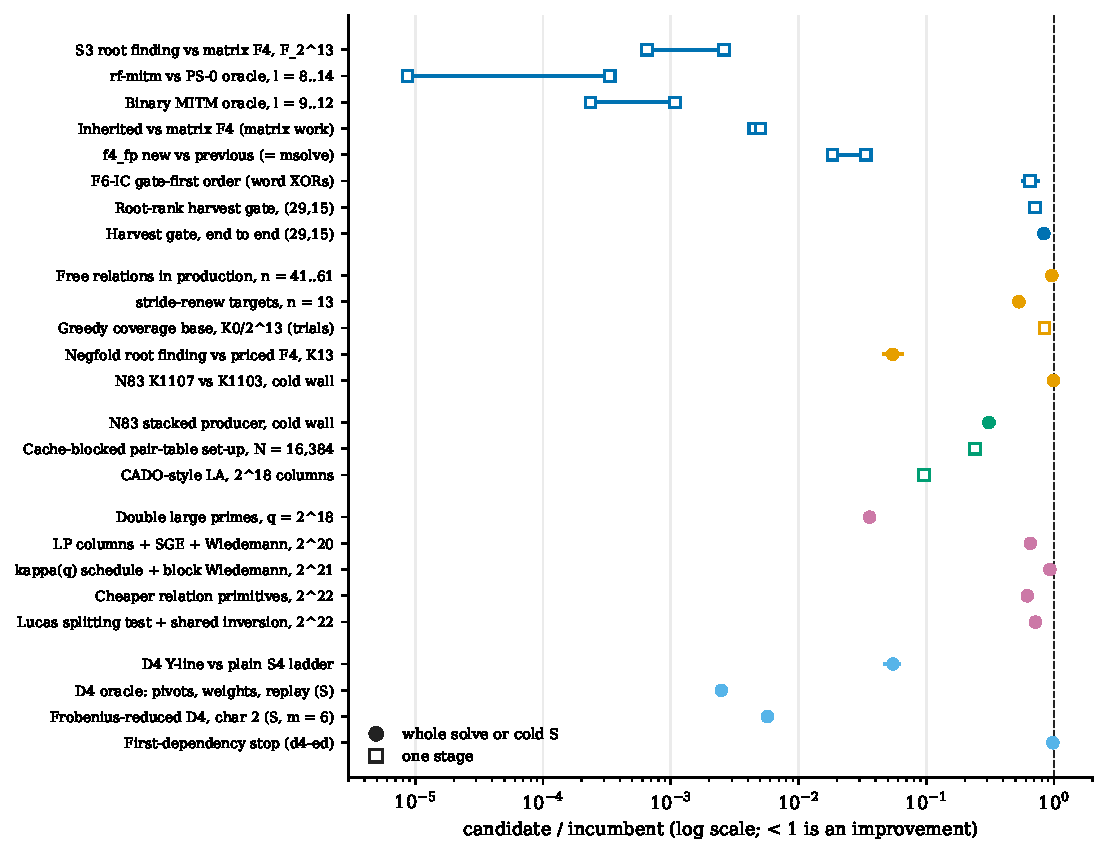
\includegraphics[width=\linewidth]{figures/fig-ratchet.pdf}
\caption[]{The ratchet. Each row is one change, candidate/incumbent on the
study's own boundary; less than 1 is an improvement. Filled circles are
whole solves or cold $S$; open squares are single stages. Bars show 95\%
intervals. Rows with two markers show the range a source reports across
instances, not an interval. Rows are grouped by pipeline term and are not
comparable across groups: incumbents, curves and units differ. Values and
sources: \art{papers/ecdlp-ic-improvement-ledger/figures/data.json}.}
\label{fig:ratchet}
\end{figure}

\subsection{Root finding replaces the Gr\"obner solve}

For two summands, the decomposition question has a closed-form answer.
For $E:y^2=x^3+ax+b$ and affine $R,F$ with $x_R\ne x_F$,
\[
  S_3(x_R,x_F,X)=(x_R-x_F)^2\,\bigl(X-x(R+F)\bigr)\bigl(X-x(R-F)\bigr).
\]
So $R=\pm F_i\pm F_j$ if and only if $x(R\mp F_i)\in x(\Fb)$. The identity is
machine-checked in Lean~4 with Mathlib
(\art{papers/rootfinding-decomposition/lean/S3Roots.lean}). The resulting
oracle is one subtraction and one hash probe per base point, with every
inversion batched. For $m=3,4$, a table of pair sums turns a decomposition
into $N$ or $N^2$ probes. The mechanism is the second algorithm of McGuire
and Mueller~\cite{mcguire2017}; what is new here is engineering and
measurement.

Per decomposition, root finding is $383\times$ ($\FF_{2^9}$, $N=55$) and
$1{,}535\times$ ($\FF_{2^{13}}$, $N=4{,}005$) cheaper than matrix F4. Every
verdict agreed with F4. The \texttt{rf-mitm} oracle refutes a binary target
$3{,}007$--$115{,}160\times$ faster than the earlier PS-0 oracle across
$\ell=8..14$ (\art{research/pdp_root_finder_20261012/}). The
meet-in-the-middle oracle on a non-Koblitz curve over $\FF_{2^{37}}$
reached $\ell=12$. It is $928$--$4{,}244\times$ faster than pairs-and-solve
on $\ell=9..12$, with no disagreement on 256 targets
(\art{research/binary_mitm_oracle_l11_l12_20261016/}).

The end-to-end effect is two orders of magnitude smaller than the stage
effect:
\begin{itemize}
\item against msolve, on 16--24-bit prime curves, $50$--$105\times$;
\item on the one binary instance large enough to amortise the table
  ($n=23$), $122\times$; F4 is faster at $n\le13$;
\item inside ecbench at Koblitz $n=13$, a root-finding arm folded over
  negation costs $0.0545$ $[0.047,0.064]$ of an inherited-F4 arm whose
  word XORs are priced (\art{research/ecbench_rootfind_faster_20261014/}).
\end{itemize}
A late correction affects the last comparison. On 20 October a cross-ISA
replay showed that F4's counted word XORs depend on whether the host has
BMI2 (\S\ref{sec:audit}). Once F4 is priced, the root-finding pair table
is about $17$--$22\times$ cheaper than F4 at $n=13$
(\art{research/validation_sweep_20261019/D-known-issues/REPORT.md}). The
direction is unchanged.

\subsection{The Gr\"obner family, where it is still needed}

For $m\ge3$ over binary fields the oracle is still a Gr\"obner solve. Four
changes moved it.
\begin{itemize}
\item \emph{Inherited F4.} Each child node of the DPLL-style tree inherits
  its parent's echelon form. This does $198.6$--$222.1\times$ less matrix
  work than matrix F4 on identical trees. At $m=19$ matrix F4 timed out at
  $1{,}800$\,s, while inherited F4 finished in about 6\,s
  (\art{research/f4_f5_f6_cross_family_20261011/}).
\item \emph{$\FF_p$ F4 at msolve parity.} Gebauer--M\"oller criteria,
  packed monomials and interned symbolic preprocessing made
  \texttt{f4\_fp} $29.8$--$54.1\times$ faster than its predecessor. msolve
  over ours is $0.96$--$1.22$ single-threaded, and every reduced basis
  agrees with Singular or msolve
  (\art{research/f4_fp_msolve_parity_20261011/}). Blocked pair reduction
  then gave $0.78$--$0.89\times$ wall on the quadratic $n=10,11$ systems
  (\art{research/f4_fp_blocked_pairs_20261016/}; L0, descriptive).
\item \emph{Gate-first order in F6-IC.} Checking the factor-base domain
  gate before reduction cuts word XORs by $1.336$--$1.733\times$ and CPU by
  $1.56$--$2.12\times$. All 80 of 80 targets were decided identically
  (\art{research/f6_gate_first_x86_20261016/}). It is now the default. An
  arm64 rerun on 22 October found that turning it off costs
  $1.62$--$2.15\times$, so every default stands
  (\art{research/arm64_f4_defaults_20261022/README.md}; shared CI VMs, one
  run each).
\item \emph{Harvesting what the oracle discarded.} Linear rows that the
  Gr\"obner oracle used to throw away are kept: $0.858$ $[0.803,0.916]$ at
  $(n,\ell)=(23,12)$, where the gate fires. A root-rank gate then made the
  harvest fire on more cells: $1.41\times$ $[1.32,1.52]$ CPU at $(29,15)$,
  $1.89\times$ at $(37,19)$, and $1.20\times$ and $1.14\times$ end to end
  at $(29,15)$ and $(31,16)$, with 0 of 248 root-set failures
  (\art{research/ic_improve3_20261015/02-harvest-gate}).
\end{itemize}

\paragraph{Changes that did not count.}
\begin{itemize}
\item \emph{F6-IC as a frontier move.} F6-IC uses $0.77$--$0.82$ of
  inherited F4's word XORs. Once its batched group additions are charged,
  though, its $S$ is $64.6$--$1{,}353\times$ inherited F4's. That is
  \cls{accounting}.
\item \emph{Algebraic oracles against the MITM floor.} No algebraic oracle
  (inherited F4, F6-IC, SAT, split-$S_4$ hybrids, a chained-$S_3$ solver)
  grows more slowly in $n$ than the meet-in-the-middle floor. The cheapest
  is $3.0\cdot10^2\times$ the floor at $n=13$ and $3.8\cdot10^4\times$ at
  $n=31$ for $m=3$ (\art{research/ic_m3_algebraic_vs_mitm_20261014/}).
\item \emph{Root-shape replay in inherited F4.} It regresses by
  $1.015$--$1.328\times$, so the switch stays off
  (\art{research/pdp_shape_replay_20261015/}).
\item \emph{F4 trace replay in the Jacobian-cover pipeline.} It now costs
  $+31\%$ and $+35\%$ (\art{research/ic_cover_leads_20261018/README.md}).
\end{itemize}

\paragraph{Reading.} The oracle is the term the programme improved most:
by two to five orders of magnitude where root finding applies, and by one to
two orders in counted matrix work where Gr\"obner bases are still needed.
None of this changes the trial count $m!\,r/N^{m-1}$. That is why the
remaining sections deal with $N$, the yield, set-up and linear algebra.

\section{The ratchet, II: factor base and relation yield}\label{sec:basis}

This section covers $N$ and $\rho_{\mathrm{yield}}$ in~\eqref{eq:cost}. On
Koblitz curves these terms are the main target, because the curve's
Frobenius gives the factor base structure the index calculus can use.

\subsection{Compact Frobenius orbits}

On $y^2+xy=x^3+ax^2+1$ over $\FF_{2^n}$ the Frobenius $\pi$ acts on the
subgroup as a scalar $\lambda$. A $\pi$-invariant base splits into orbits
with $\log\pi^k(P)=\lambda^k\log P$, so the unknowns collapse by about
$n$~\cite{ggmp2020}. The programme's \emph{compact signed-Frobenius orbit}
base stores one representative per orbit and no pair table
(\art{docs/ic/COMPACT_ORBIT_PRODUCER.md}). It is the best measured Koblitz
construction:
\begin{itemize}
\item in the ecbench factor-base suite at $n=17$ it is $9.985\times$
  matched signed-Frobenius rho, against $18.7\times$ for full orbits and
  $47\times$ for subspace bases (\art{research/ecbench_frontier_20261013/});
\item in the priced frontier campaign it is $3.8$--$15\times$ rho at $w=0$
  and $4.9$--$17.8\times$ at $w=0.1$ on eight Koblitz curves
  (\art{research/ic_frontier_campaign_20261015/});
\item fully priced against fully priced signed-Frobenius rho, its best cell
  is $1.566$ $[0.992,2.347]$. That interval reaches 1, but the ratio is
  never below 1, and the fitted gap grows as $r^{0.165\,[0.117,0.213]}$
  (benchmarks row \texttt{20261014-frobenius-orbit-ic-vs-rho}; 2{,}816 of
  2{,}816 records verified).
\end{itemize}

\subsection{Free relations and re-randomised targets}

\begin{itemize}
\item \emph{Free relations.} Self-collisions in the root table are used as
  homogeneous rows. In production at $n=41,53,61$ this gives $0.960$
  $[0.946,0.976]$ counted and $0.941$ in wall. A census closes the lever,
  though: at $n=61$, $K=600$ the self-collisions span only 49 of the 599
  relations needed. Full rank from free relations alone would need
  $K\approx2{,}050$ (benchmarks row
  \texttt{20261014-ic-next10-09-equal-advice}).
\item \emph{\texttt{stride-renew} targets.} Re-randomising the target
  combination at a fixed stride instead of walking it gives $0.531$
  $[0.506,0.557]$ at Koblitz $n=13$. The result is $4.7\times$ strong rho
  at $n=19$ (benchmarks row \texttt{20261014-rootfind-stride-targets}).
\end{itemize}

\subsection{Choosing the base}

\begin{itemize}
\item \emph{Greedy coverage.} A base chosen greedily to maximise
  decomposable coverage needs $4.46$ expected trials instead of $5.29$ on
  $K_0/2^{13}$, a ratio of $0.843$. The gain decays with size: $1.090$ at
  $r=2^{16}$ and $1.0000$ at $r=2^{39}$
  (\art{research/greedy_factor_base_yield_20261014/}). It is a real stage
  improvement that does not reach cryptographic sizes.
\item \emph{$n=83$ base selection.} At Koblitz $n=83$ the cold pipeline's
  base was re-selected on 16 fresh public points under a frozen protocol.
  Base K1107/root11 has a mean cold process of $113.755$\,s against
  $114.950$\,s for K1103. That is a paired reduction of $1.195$\,s
  $[0.957,1.433]$, and every one of the 16 per-point differences favours
  K1107. All 64 IC arms and 16 rho arms were admitted on a GitHub Tier~1
  host, and a second local verifier reproduced the analysis exactly
  (\art{research/n83_cold_base_confirm_20261021/RESULT.md}). It is small
  ($0.990\times$) but verified, and it is the current $n=83$ cold baseline.
  Rho was measured online only in this study (geometric mean
  $2{,}334.964$\,ms), so it has no cold IC/rho ratio of its own. The last
  cold ratio at $n=83$ is the earlier holdout's $55.368$ (K1120,
  \S\ref{sec:distance}).
\item \emph{Kummer-tower bases over $\FF_p$.} The $\mu_{2^t}$ bases of
  Petit, Kosters and Messeng~\cite{pkm2016} cost the same as a plain base
  of the same size to within 1\% (ratios $0.999$--$1.012$) under root
  finding. Their structure helps an algebraic solver, not a table
  (\art{research/pkm_tower_ecbench_20261013/}). This is a null result.
\end{itemize}

\paragraph{Refuted or neutral.} Three bases or filters did not help:
\begin{itemize}
\item a cyclotomic $\gamma$-weighted base, at $1.022$ $[1.021,1.023]$;
\item a trace-zero pre-filter, at $1.00003$, which is vacuous on odd order;
\item symmetrised $u$-frame bases, which saved $0.76$--$0.84\times$ at
  $n=17,23$ but cost $4.01\times$ at $n=31$
  (\art{research/koblitz_symmetrised_e2e_20260927/}).
\end{itemize}

\paragraph{Reading.} Every change in this section is \cls{engineering} in
the constant. None changes how the relation count scales with $r$, and the
Koblitz gap to rho still grows as roughly $r^{1/6}$ (\S\ref{sec:distance}).
The open lever is the yield per probe at fixed $N$.

\section{The ratchet, III: set-up and linear algebra}\label{sec:setup}

\subsection{Set-up}

Set-up is the largest term on the Koblitz pipelines (\S\ref{sec:model}).
\begin{itemize}
\item \emph{Stacked $n=83$ producer} (\texttt{cryptanalysis} \#938). This
  stacks the cryptanalysis repository's set-up optimisations into one
  producer. It made end-to-end cold $3.2391\times$ $[2.9809,3.5240]$
  faster than its own baseline. Paired within that run, the cold gap to
  rho fell from $305.8$ to $94.4$. The online ratio moved from $0.133$ to
  $0.139$, a small online regression. An integrity audit upheld the claim
  within a narrower scope (\art{crypto-autoresearcher:research/sheriff/SHF-20261016-3caa6f/findings.yaml},
  C17--C19):
  \begin{itemize}
  \item it is one run on one runner class, with no replay on another host;
  \item about $1.48\times$ of the gain is host-independent operation
    counts, and the rest is wall time;
  \item factor-base construction is charged to neither arm;
  \item the repository's ``$360\to94.4$'' wording and a set-up field
    compared across rows with different meanings were judged
    overclaimed.
  \end{itemize}
  We report the scoped figure.
\item \emph{Cache-blocked pair table.} Building the prime-field pair table
  in cache-sized blocks cuts set-up to $0.24$ $[0.22,0.26]$ of the batched
  build and $0.13$ $[0.12,0.14]$ of the scalar build at $N=16{,}384$. That
  is $28.2$\,s instead of $117$\,s and $224$\,s, and peak memory falls from
  $9.15$\,GiB to $4.65$\,GiB. All 456 of 456 executions are identical, and
  the A/A ratio is $1.02$ $[0.70,1.46]$
  (\art{research/ic_oracle_setup_blocked_20261020/}). Two caveats apply.
  The host earned L1, so the wall ratios are descriptive. And counted $S$
  is unchanged, so this is a wall-time gain that leaves the gap in the
  counted unit as it was (rho is $32.96$, $74.31$ and $269.03\times$
  cheaper at $N=1{,}024$ to $16{,}384$, $w=0$).
\item \emph{u64 root batching.} Batching root extraction in 64-bit lanes
  gives $3.26\times$ whole-process. The rank-stage and per-target cells were
  corrected on 20 October from $2.95\times$ and $6.09\times$ to $2.47\times$
  and $5.00\times$; the originals had compared the candidate's fastest run
  with the baseline median (benchmarks row \texttt{20261015-u64-rootbatch}).
\end{itemize}

\subsection{Linear algebra}

\begin{itemize}
\item \emph{CADO-style filtering and Wiedemann.} On synthetic $m=3$
  matrices over a 62-bit prime, a filter followed by
  Wiedemann~\cite{wiedemann1986} beats the legacy solver by $2.48\times$
  at $2^{14}$ columns and $10.40\times$ $[9.99,11.06]$ at $2^{18}$. At
  $2^{18}$ it is $1.93\times$ $[1.74,1.96]$ faster than CADO-NFS itself
  (\art{research/la_engines_20261014/}).
\item \emph{Inside ecbench.} Wired into the end-to-end pipeline, the same
  solver leaves counted $S$ at $1.000$ and cuts linear-algebra wall time
  to $0.25$--$0.72$. Linear algebra is only 0.1--1.9\% of these runs, and
  the best cell is still $149\times$ rho
  (\art{research/ic_linalg_pipeline_20261019/}).
\item \emph{Deferred sparse solvers.} A negative: no deferred sparse
  solver lowers end-to-end $S$ ($1.206\times$ on the $k=4$ ladder;
  $5.72\to1.030\times$ on the scaling curve). These solvers answer only at
  full rank, which is a completion-rule effect, not a linear-algebra one
  (\art{research/sparse_la_timing_20261018/README.md}).
\item \emph{Sparse FGLM in the Jacobian-cover pipeline} cuts $S$ by
  $1.28$--$1.29\times$. For example, IC/rho falls from $851$ to $664$ at
  $p=53$ (\art{research/jv_cover_sparse_fglm_20261018/}). Both are lower
  bounds.
\end{itemize}

\paragraph{Reading.} The set-up results are the largest end-to-end
constant-factor gains of the period: $3.24\times$ at $n=83$, and $4$--$8\times$
in prime set-up wall. Linear algebra is a large stage gain on a term that
is small on the curves measured. It becomes the term that matters on the
genus-three family (\S\ref{sec:families}), where large primes and
structured Gaussian elimination moved the exponent.

\section{The ratchet, IV: families where the exponent moves}\label{sec:families}

Two families have a fitted cost exponent below rho's. On both, the ratchet
moved fastest. Neither is a deployed curve shape.

\subsection{Genus three after the cubic GHS transfer}

The GHS Weil descent~\cite{ghs2002} maps the discrete logarithm in
$E_0(\FF_{q^3})$ to the Jacobian of a genus-three hyperelliptic curve over
$\FF_q$. There, double-large-prime index calculus~\cite{gtthd2007} costs
$\tilde O(q^{2-2/g})=\tilde O(q^{4/3})$, against rho's $q^{3/2}$ on
$E_0(\FF_{q^3})$. The asymptotics are known. The programme contributes a
priced, end-to-end, verified implementation:
\begin{itemize}
\item the family has $4\mid\#E_0(\FF_{q^3})$, split arm;
\item it runs for $q=2^{8}$ to $2^{22}$;
\item every logarithm is checked against the planted scalar;
\item cost is counted in $\FF_q$ multiplications, with inversions charged
  from round three on.
\end{itemize}
Five rounds, each against the previous one's frozen incumbent:

\begin{enumerate}
\item \emph{Double large primes} (Ie): $q^{1.910}\to q^{1.385}$
  $[1.379,1.391]$, and $0.036$ $[0.035,0.036]$ of the full-base incumbent at
  $q=2^{18}$ (benchmarks row \texttt{20261014-ic-improve-04-genus3-2lp}).
\item \emph{Large primes kept as columns, structured Gaussian elimination
  and Wiedemann} (Ie): $q^{1.398}\to q^{1.380}$, $0.653$ $[0.647,0.660]$ at
  $q=2^{20}$.
\item \emph{A frozen schedule $\kappa(q)$ for the factor-base fraction, plus
  block Wiedemann}~\cite{coppersmith1994} (T): $0.929$ at $q=2^{21}$; with
  round two, $0.605\times$ the first double-large-prime arm. After this
  round a matched negation-map rho was measured at $q=2^{20}$: IC costs
  $2.31\cdot10^{10}$ $\FF_q$ multiplications against rho's $2.01\cdot10^{10}$,
  i.e.\ $1.15\times$ (overlapping but not identical curves).
\item \emph{Cheaper relation primitives} (Ic): one-inversion Cantor
  addition, a Stickelberger pre-filter and reused exponentiations, with
  $\kappa$ re-tuned. The result is $0.617$ $[0.616,0.619]$ at $q=2^{22}$,
  without changing a single relation
  (\art{research/ic_improve3_20261015/01-genus3-relations}).
\item \emph{A Lucas-ladder splitting test} on the Cardano resolvent's cubic
  character, plus 32 walks sharing one inversion (Ie, then Ic). The
  per-trial log factor falls from 9.75 to 2.71 units per bit. The whole
  solve is $0.756$ $[0.755,0.756]$, then $0.715\times$, at $q=2^{22}$; the
  local exponent is $1.356$, and the fit over $2^{16}$--$2^{22}$ is $1.368$
  (\art{research/ic_improve4_20261015/01-genus3-relations}).
\end{enumerate}
Chained, rounds three and four bring the whole solve to about $0.44\times$
the round-two pipeline at $q=2^{22}$. This is derived, in the
inversion-charging unit.

\paragraph{Distance.} The last matched distance is $1.15\times$ rho at
$q=2^{20}$, after round two. Rounds three and four ran no rho arm in their
unit. Whether the $0.44\times$ carries the family across rho is therefore
\emph{not established}, and we do not claim it.
\begin{itemize}
\item A separate study measured IC at $0.16\times$ a rho on
  $\mathrm{Jac}(C)$ at $q=2^{14}$. That rho walks on the Jacobian, not on
  $E_0(\FF_{q^3})$, so it is not the matched reference.
\item The local exponents ($1.36$--$1.41$) sit above $4/3$. The linear
  algebra grows faster than $q^{4/3}$, and re-tuning $\kappa$ steepens the
  schedule.
\item Memory now bounds the ladder: $q=2^{22}$ peaks at 3.9\,GB of a
  4.5\,GB cap.
\end{itemize}

\subsection{$k=4$: Gaudry's index calculus with FGHR symmetry}

Over $\FF_{p^4}$ with a base of points whose abscissa lies in $\FF_p$, each
relation needs a four-term decomposition~\cite{gaudry2009}. On a curve with
rational 2-torsion $T$, the coordinate $Y$ with $Y(P+T)=-Y(P)$ makes $S_5$
invariant under the Weyl group $D_4$, of order 192~\cite{fghr2014}. The
ratchet on this family:
\begin{enumerate}
\item \emph{$D_4$ invariants} (E): the Macaulay matrix shrinks from
  $41{,}780\times40{,}920$ to $13{,}412\times11{,}628$. One decomposition
  costs $47.5$--$48.4\times$ less at $p=269$
  (\art{research/gaudry_quartic_d4_20261013/}).
\item \emph{$D_4$ $Y$-line on a complete ladder} (Ic): $0.0548$
  $[0.048,0.061]$ of plain $S_4$ on $p=101$--$1033$, 21 curves.
\item \emph{Sparsest pivots, the weighted grading $\sigma_4=\pi^2$, shape
  replay} (E/Ic): $C_4$ falls from $2.55\cdot10^{10}$ to $6.89\cdot10^7$
  $\FF_p$ multiplications ($369.8\times$ $[367.9,371.6]$; 648 of 648 solves
  exact). Ecbench $S$ falls $398$--$406\times$
  (\art{research/gaudry_quartic_d4_cost_20261014/}).
\item \emph{First-dependency stop} (Ic): $0.979$ $[0.973,0.986]$. Double
  large primes cut the linear algebra to $0.827\times$ but regress the
  whole solve ($1.025\times$).
\item \emph{A Frobenius-reduced $D_4$ form in characteristic two} (E/Ic):
  weights $(2,2,1,1)$, Macaulay degree 11, a $384\times448$ matrix. It is
  $481\times$ below the plain form at $m=8$, and ecbench $S$ is $0.0057$ of
  the plain form at $m=6$ (\art{research/gaudry_quartic_d4_char2_20261015/}).
\end{enumerate}

\paragraph{Distance.} The two characteristics are far apart.
\begin{itemize}
\item Over $\FF_{p^4}$ index calculus is still $1.39\cdot10^6\times$ rho at
  the measured sizes.
\item Over $\FF_{(2^m)^4}$ the gap closes with size
  (Figure~\ref{fig:families}). IC over the negation-map rho model is
  $5{,}080$ at $m=6$ ($n\approx2^{24}$), $648$ at $m=8$, $80.6$ at $m=10$,
  $49.7$ at $m=12$ and $6.06$ at $m=14$ ($n\approx2^{56}$). Against a
  measured rho the last value is $4.27$, from a single target. The fitted
  slope is $-0.248$ in $\log_2 n$, which is Gaudry's $n^{-1/4}$. The
  extrapolated crossover is near $n\approx2^{68}$, where rho takes about
  $2^{34}$ steps, so the extrapolation can be tested directly.
\end{itemize}
After genus three, this is the nearest any index calculus in the programme
has come to rho.

\paragraph{Joux--Vitse.} An $(n-1)$-decomposition~\cite{jouxvitse2012} at
$n=5$ over $E(\FF_{p^5})$ completed verified logarithms at
$4.5\cdot10^7$--$1.8\cdot10^8\times$ rho
(\art{research/joux_vitse_n1_20261015/}). It is a route reproduction, not an
improvement.

\subsection{The ledger in one table}

Table~\ref{tab:ledger} lists every improvement of
\S\S\ref{sec:oracle}--\ref{sec:families} that changed a default or a
baseline, with its class and the distance to rho that remained after it.

\begin{table}[p]
\centering\small
\caption[]{The ratchet: changes that became the new incumbent, July--October
2026. Ratio is candidate/incumbent. Class against the IC incumbent: Ie
exponent, Ic constant, E one stage, T trades. Boundary: St stage, Cx
complete, Cd cold. ``To rho'' is IC/matched rho after the change, on the
study's own boundary; a dash means no matched rho in that unit. Every
row's IC answers were verified. ``d'' marks a derived reciprocal.}
\label{tab:ledger}
\begin{tabularx}{\linewidth}{@{}>{\raggedright}Xlll>{\raggedright\arraybackslash}p{2.5cm}@{}}
\toprule
Change & Cl. & Bd. & Ratio [95\%] & To rho \\
\midrule
\multicolumn{5}{@{}l}{\emph{Oracle}}\\
$S_3$ root finding vs matrix F4 & E & St & $1/1{,}535$--$1/383$ & --- \\
Inherited vs matrix F4 & E & St & $1/222$--$1/199$ & --- \\
\texttt{f4\_fp} to msolve parity & E & St & $1/54.1$--$1/29.8$ & --- \\
Negfold root finding vs priced F4, K13 & Ic & Cd & $0.0545$ $[0.047,0.064]$ & $1.55\times$ strong rho \\
F6-IC gate-first & E & St & $0.65$ $[0.58,0.75]$ & --- \\
Root-rank harvest gate & Ic & Cx & $1/1.20$ (St $1/1.41$) & --- \\
\addlinespace
\multicolumn{5}{@{}l}{\emph{Factor base and yield}}\\
Free relations in production & Ic & Cx & $0.960$ $[0.946,0.976]$ & $3.8$--$15\times$ ($w=0$) \\
\texttt{stride-renew} targets, $n=13$ & Ic & Cd & $0.531$ $[0.506,0.557]$ & $4.7\times$ at $n=19$ \\
N83 base K1107 vs K1103 & Ic & Cd & $0.990$ (d; $-1.195$\,s $[0.957,1.433]$) & $55.4\times$ (K1120) \\
\addlinespace
\multicolumn{5}{@{}l}{\emph{Set-up and linear algebra}}\\
N83 stacked producer & Ic & Cd & $1/3.24$ $[1/3.52,1/2.98]$ & $94.4\times$ (in-run) \\
Cache-blocked pair table (wall, L1) & E & St & $0.24$ $[0.22,0.26]$ & $33$--$269\times$ \\
CADO-style LA, $2^{18}$ columns & E & St & $1/10.40$ $[1/11.06,1/9.99]$ & $149\times$ \\
\addlinespace
\multicolumn{5}{@{}l}{\emph{Genus three after cubic GHS ($\FF_q$ multiplications)}}\\
Double large primes & Ie & Cx & $0.036$; $q^{1.910}\to q^{1.385}$ & $2.58\times$ model \\
LP columns, SGE, Wiedemann & Ie & Cx & $0.653$ $[0.647,0.660]$ & --- \\
$\kappa(q)$ + block Wiedemann & T & Cx & $0.929$ & $1.15\times$ measured \\
Relation primitives & Ic & Cx & $0.617$ $[0.616,0.619]$ & --- \\
Lucas splitting + shared inversion & Ie/Ic & Cx & $0.715$; local $1.356$ & --- \\
\addlinespace
\multicolumn{5}{@{}l}{\emph{$k=4$ with $D_4$ symmetry}}\\
$D_4$ $Y$-line ladder & Ic & Cx & $0.0548$ $[0.048,0.061]$ & model handover $2^{126}$--$2^{137}$ \\
Pivots, weights, replay ($S$) & Ic & Cd & $0.00249$ $[0.00246,0.00251]$ & $1.39\cdot10^6\times$ \\
First-dependency stop & Ic & Cx & $0.979$ $[0.973,0.986]$ & --- \\
Frobenius-reduced form, char.\ 2 ($S$) & Ic & Cd & $0.0057$ & $6.06\times$ model, $4.27\times$ measured, $n\approx2^{56}$ \\
\bottomrule
\end{tabularx}
\end{table}

\section{The distance that remains}\label{sec:distance}

This section reports IC/rho, with greater than 1 meaning rho is cheaper. It
gives the current figure for each family, the reference it uses, and how
that figure moved over the period.

\begin{figure}[t]
\centering
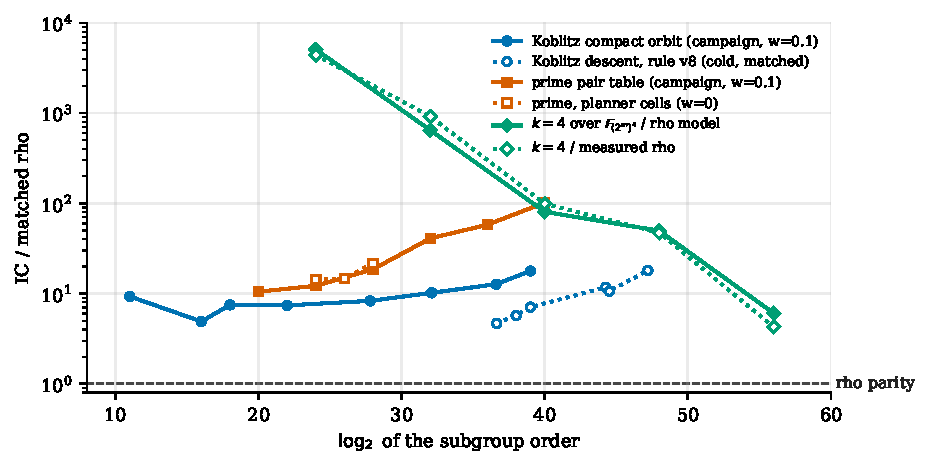
\includegraphics[width=\linewidth]{figures/fig-families.pdf}
\caption[]{Distance to matched rho by family and size. Koblitz and prime
curves use the frontier campaign's priced arms ($w=0.1$, 16 targets
$\times$ 2 rounds) and, open markers, the Koblitz rule at v8 (cold, 64
targets) and the prime planner cells ($w=0$). $k=4$ over $\FF_{(2^m)^4}$
uses the char-2 ladder against the negation-map rho model (filled) and a
measured rho (open); the $n\approx2^{56}$ point is one target. Curves and
units differ between families, so the lines are not ranked against each
other. Sources: \art{figures/data.json}.}
\label{fig:families}
\end{figure}

\subsection{Koblitz curves: the rule at a matched rho}

The leaderboard's Table~A measures a Koblitz descent (aimed $m=3$
collection, $m=2$ or $m=3$ descent) cold on one unseen public point per
process: 64 points per size and six sizes from $2^{36.6}$ to $2^{47.2}$.
It was re-run three times on the same instances
(\art{research/ic_tool_program/rule/}), and Figure~\ref{fig:koblitz} shows
all three.
\begin{itemize}
\item \emph{v3 to v7: an IC improvement.} With the same rho, IC became
  $1.52$--$1.89\times$ faster (\#1978), and the cold ratio fell from
  $5.23$--$20.97$ to $3.43$--$11.51$.
\item \emph{v8: a matched reference.} The rule was run on one binary with
  rho's signed-Frobenius canonicalisation batched 16 lanes wide, against a
  same-binary control with rho as at v7. In both runs 408 of 408 rows pass
  the \texttt{vs\_rho} check, and the matched rho takes the same walks as
  the control on 64 of 64 targets per size. IC's online time is unchanged
  between runs ($0.976$--$1.033$). Rho's online time fell $1.42$--$1.62\times$.
  The cold gap against the matched rho is
  \[
    4.67\,[4.34,5.07],\ 5.70,\ 7.07,\ 11.75,\ 10.65,\ 18.07\,[15.98,20.58]
  \]
  at $\log_2 r=36.6, 38.0, 39.0, 44.3, 44.5, 47.2$. All six values lie
  inside ranges declared before the rows were taken
  (\art{research/ic_tool_program/rule/v8/README.md}).
\end{itemize}
Two readings follow, and both hold.
\begin{itemize}
\item The $1.52$--$1.89\times$ IC improvement is real and \cls{engineering}.
\item Against the matched rho, v8's distance sits about where v3's sat
  against the old rho. The fitted slope of the gap is $0.168$ $[0.128,0.208]$
  per $\ln r$, against v3's $0.176$. The apparent flattening between v3 and
  v7 was mostly an artefact of an unmatched rho. The class of v8 is
  \cls{engineering} on the rho side and \cls{accounting} for the gap.
\end{itemize}
Pricing rho at its canonical step instead of as built gives a model gap of
$6.45$--$23.32\times$. The validation sweep, recomputing Table~A's rows that
way, reads $9.13$--$41.13\times$
(\art{research/validation_sweep_20261019/A-leaderboard/REPORT.md}). The
leaderboard still prints the v3 ratios; the v8 figures supersede them as the
distance remaining.

\begin{figure}[t]
\centering
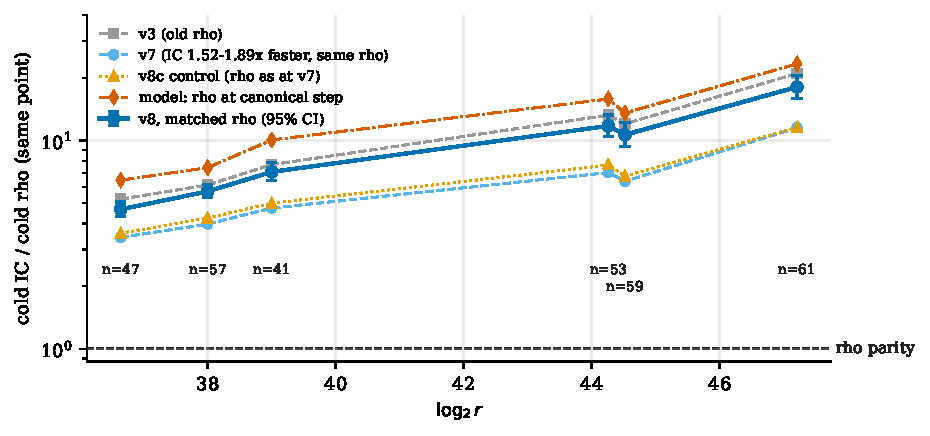
\includegraphics[width=\linewidth]{figures/fig-koblitz-rule.pdf}
\caption[]{The Koblitz rule at three baselines, cold IC over cold rho on the
same public point, 64 targets per size. v3 to v7 is an IC improvement with
the same rho; v8 is the same IC against a matched (faster) rho, with a
same-binary control (v8c) that reproduces v7. The dash-dot line prices rho
at the canonical step. Source:
\art{research/ic_tool_program/rule/v8/README.md}.}
\label{fig:koblitz}
\end{figure}

\paragraph{The priced campaign.} The frontier campaign
(\art{research/ic_frontier_campaign_20261015/}) ran every method family on
the same fixed ladders, with 16 public targets per curve and every native
operation priced across the band. Of its 4{,}848 executions, 3{,}178
measured runs were verified, and 19 of 19 replay audits were identical. The
closest Koblitz arm, compact orbit, is $3.8$--$15\times$ signed-Frobenius
rho at $w=0$ and $4.9$--$17.8\times$ at $w=0.1$. Its fitted exponent on
$n=37$--$47$ is $0.589$ $[0.518,0.743]$, against rho's $0.436$
$[0.358,0.508]$, separated at $w=0$ only.

\paragraph{$n=83$.} The last cold measurement is the 16 October holdout
with K1120, on five public points: IC at $119.826$\,s cold against
rho's mean $2.164$\,s on the same points, a ratio of
$55.368$ (\art{research/n83_e2e_holdout_20261016/RESULT.md}). Its frozen
selection is \texttt{BOUNDED\_UNKNOWN}. K1107 since cut $1.195$\,s from a
$115$\,s process (\S\ref{sec:basis}), which moves this ratio by about 1\%.
The stacked producer's in-run gap of $94.4$ uses a different baseline and
rho measurement (\S\ref{sec:setup}). Two $n=83$ baselines in the
\texttt{crypto} and \texttt{cryptanalysis} repositories ($120$\,s and
$195.7$\,s) are not yet reconciled.

\subsection{Prime curves}

\begin{itemize}
\item \emph{Campaign.} The two-summand pair-table arm goes from $10.5\times$
  rho with negation at 20 bits to $101.8\times$ at 40 bits ($w=0.1$). Its
  fitted exponent is $0.620$ $[0.557,0.663]$, against rho's $0.435$, which
  is the $r^{2/3}$ against $r^{1/2}$ of \S\ref{sec:model}. The Kummer-tower
  arm is $28$--$159\times$.
\item \emph{Planner.} A cost-model planner chose the base and arity per
  curve, and was validated on six registered and three supplementary prime
  curves. The plan beats every alternative arm at $w=0$, and rho is
  cheaper on every curve, by $12.6$--$25.8\times$. The best registered cell
  is $14.39$ $[11.63,18.45]$ at 24 bits, against a predicted $12.23$
  (1{,}152 runs, all verified, 72 exact replays;
  \art{research/ic_planner_validation_20261020/README.md}).
\item \emph{ECCp-131.} Exact relation paths were built for the Certicom
  ECCp-131 parameters, as a correctness exercise. Every arm found zero
  relations: a two-sum probe at $B=512$ and a three-point probe whose hit
  probability is at most $2^{-106.19}$ at $B=128$. The 20-bit ecbench
  control on the same code path, a different curve, is $9.41$
  $[7.22,12.93]\times$ rho
  (\art{research/eccp131_bsgs_ic_20261020/REPORT.md}).
\end{itemize}

\subsection{Nearest approaches}

Table~\ref{tab:nearest} collects the smallest IC/rho the programme has
measured, with the qualifier each one carries. No entry is below 1 on an
elliptic curve with a matched cold reference.

\begin{table}[t]
\centering\small
\caption[]{Smallest measured distances to rho, by family.}
\label{tab:nearest}
\begin{tabularx}{\linewidth}{@{}>{\raggedright}p{3.6cm}l>{\raggedright\arraybackslash}X@{}}
\toprule
Family & IC/rho & Qualifier \\
\midrule
Genus 3 via cubic GHS, $q=2^{20}$ & $1.15$ & measured negation rho; overlapping, not identical curves; two later rounds ($0.44\times$) unmatched \\
$k=4$, $\FF_{(2^m)^4}$, $m=14$ & $4.27$ & one target; $6.06\times$ the rho model; closing as $n^{-1/4}$ \\
Koblitz, fully priced orbit & $1.566$ $[0.99,2.35]$ & best cell of a ladder; ratio never below 1; grows as $r^{0.165}$ \\
Koblitz rule v8, $2^{36.6}$ & $4.67$ $[4.34,5.07]$ & cold, matched, 64 targets \\
Prime, 20 bits & $10.5$ & campaign, $w=0.1$; $r^{1/6}$ widening \\
Prime, planner 24 bits & $14.39$ $[11.63,18.45]$ & $w=0$ \\
Koblitz $n=83$ & $55.4$ & cold, K1120, \texttt{BOUNDED\_UNKNOWN} \\
\bottomrule
\end{tabularx}
\end{table}

\section{Claims that did not survive}\label{sec:audit}

A ratchet is worth only as much as its pawl. Several recorded results were
corrected once the reference was matched, native work was priced, or the
evidence was replayed. Each correction is recorded in the source with a
dated note; frozen evidence is never rewritten. Figure~\ref{fig:audit}
shows the before and after values. Every correction moved IC's position
against rho \emph{down}, and several moved it from apparently ahead of rho
to behind it.

\begin{figure}[t]
\centering
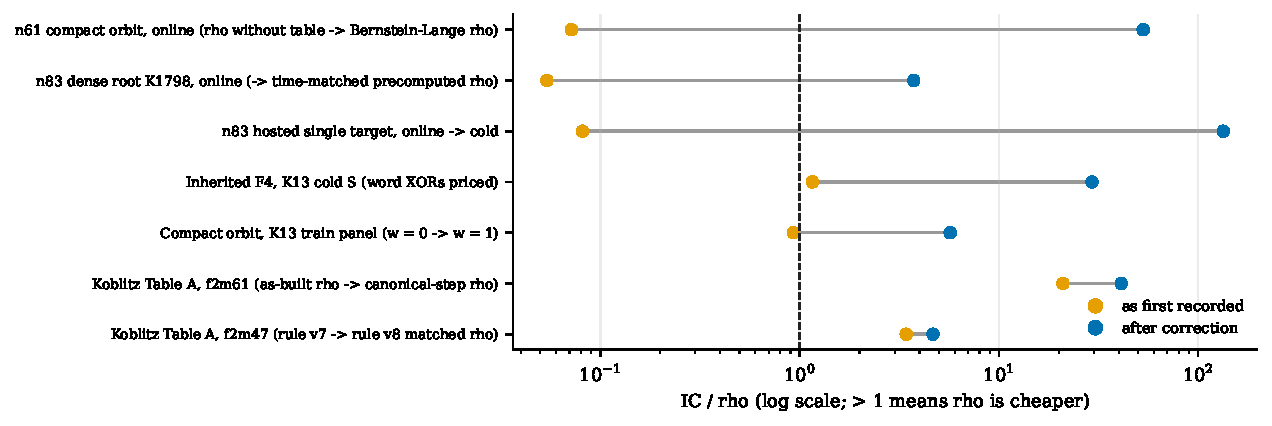
\includegraphics[width=\linewidth]{figures/fig-audit.pdf}
\caption[]{IC/rho as first recorded (orange) and after correction (blue), on
the boundary the correction used. Values left of the dashed line had
claimed IC ahead of rho. Sources: \art{figures/data.json}.}
\label{fig:audit}
\end{figure}

\paragraph{1. Every online win is retired.} The one-target online ladder
compared IC \emph{with} a retained table against rho \emph{without} one:
\begin{itemize}
\item $13.94\times$ $[9.81,19.13]$ over strong rho at $n=61$, on 64 targets;
\item $18.53\times$ at $n=83$ with a dense root index;
\item $7.29\times$ and $12.29\times$ on hosted single targets at $n=71$
  and $n=83$.
\end{itemize}
Given a distinguished-point table no larger than IC's pair table,
Bernstein--Lange preprocessing rho~\cite{bl2012} is $53$--$317\times$ faster
online at $n=41,53,61$ on the same 64 targets (benchmarks row
\texttt{20261014-ic-next10-09-equal-advice}). At $n=83$, rho with a table
matched to IC's set-up time or memory wins every pair: $3.74\times$
time-matched and $40.61\times$ memory-matched against K3300, and
$81.5$--$395.5\times$ against K600 (benchmarks row
\texttt{20261016-n83-precomputed-rho-control}). Cold, the hosted $n=83$
point is $133.7\times$ rho. Those online rows measured what a table buys,
and generic rho buys more per byte. The within-IC result survives: K1798's
probe reduction over K1500 at $n=83$ (from $300{,}021.9$ to $169{,}069.8$
probes per relation).

\paragraph{2. Pricing native work moved two arms.}
\begin{itemize}
\item \emph{Inherited F4 at $n=13$.} Its $S=16.7$, close to rho's $14.4$,
  left its Boolean word XORs unpriced. Priced, $S=421.4$
  (\art{research/ecbench_rootfind_faster_20261014/}).
\item \emph{F4 pricing change.} The pricing change (\#1774, $0.002304$ GAE
  per word XOR) made every earlier F4 $S$ a lower bound. A separate
  algorithmic change (\#1862) raised counted work
  (\art{research/f4_pricing_jump_20261018/README.md}).
\item \emph{Compact orbit at $n=13$.} Earlier quoted at $1.08\times$ rho as a
  lower bound, it reads $0.93$, $1.53$ and $5.7\times$ the strong rho at
  $w=0,0.1,1$, so the pair is unresolved inside the band
  (\art{research/ic_frontier_campaign_20261015/select/SELECTION.md}).
\end{itemize}

\paragraph{3. Matching the rho reference.}
\begin{itemize}
\item \emph{Rule v8.} Matching the rho reference raised the Koblitz gap by
  $1.30$--$1.58\times$ at every size (\S\ref{sec:distance}).
\item \emph{The standing rho improved.} Ecbench's standing
  \texttt{rho.signed\_frobenius\_strong} now runs at $0.802\times$ its
  former instruction count with identical GAE, and the strong Koblitz rho
  executes 718 instructions per step instead of 1{,}196. Counted-unit
  comparisons are unaffected. Wall-time comparisons against the older rho
  overstate IC by up to that factor.
\item \emph{Two rho studies on the prime side.} Choosing the better of
  $P\pm R$ cuts steps by $1.129\times$. Signed $\sigma$ steps on
  ECC2K-130 cut GPU time to $0.961$--$0.970$. Neither is yet in a campaign
  arm.
\end{itemize}

\paragraph{4. A replay regression, and its root cause.} The root-finder
ecbench session was recorded with a replay certificate of 120 of 168
identical records; the 48 mismatches were all in inherited F4's word-XOR
counts. On current \texttt{main} it replayed only 72 of 168, with
mismatches in all four IC arms. The validation sweep of 19--20 October
isolated the cause (\art{research/validation_sweep_20261019/D-known-issues/item1_cross_isa_20261020/RESULT.md}):
\begin{itemize}
\item \emph{Cause.} The x86-only BMI2 word-wise rewrite in
  \art{src/cryptanalysis/inherited_f4.rs} charges a different word-XOR
  count from the portable path, for example $301{,}961$ against
  $300{,}531$. The method identity does not record which path ran.
\item \emph{Confirmation.} With that branch disabled, x86 reproduces all
  168 of 168 records. An aarch64 build under emulation also reproduces 168
  of 168. An independent rerun repeated the result.
\item \emph{What it rules out.} Compiler version, source drift since the
  archive, and the two later pricing changes.
\end{itemize}
Scalars, trial counts and charged GAE outside F4 are unaffected. F4 $S$ is
not comparable across instruction-set architectures unless the path is
stated. Until the method identity records the path, the root-finder rows
rest on the original receipt.

\paragraph{5. Reported cells that compared unlike statistics.} The
u64-rootbatch rank and per-target cells compared a fastest run with a
median, and were corrected from $2.95\times$ and $6.09\times$ to $2.47\times$
and $5.00\times$ (\S\ref{sec:setup}). The $n=83$ stacked producer's
``$360\to94.4$'' cold-gap history mixed a ratio from another run; paired
within the run it is $305.8\to94.4$ (\S\ref{sec:setup}).

\paragraph{6. Results resting on faulty code or wrong references.}
\begin{itemize}
\item \emph{Plane-quartic IC.} Its $S$ values of $650{,}896$ to
  $3.79\cdot10^7$ rest on a degree-3 reduction in
  \art{research/ghs_cubic_quartic_ic_20261012/quartic_ic.rs} that merges
  distinct classes (reported in an open pull request). Recoveries are still
  checked against the planted scalar, but relation counts and $S$ are
  unverified.
\item \emph{Volcano census crater.} A claim that IC is 22--25\% cheaper on
  the volcano crater was withdrawn, because the crater's rho reference
  should have been the cubic-automorphism rho. Against it, IC is
  $84.9\times$ rho at $w=0$
  (\art{research/volcano_ecdlp_census_20261017/REPORT.md}, erratum A3).
\end{itemize}

\paragraph{Reading.} None of these corrections removes an IC improvement
against its own incumbent. They correct the \emph{distance to rho}, which
is the quantity most exposed to an unmatched reference or an unpriced
counter. This is why the gate of \S\ref{sec:gate} asks for a matched,
band-priced rho on every row.

\section{Validation status}\label{sec:gate}

As of 23 October 2026, \textbf{no index-calculus leaderboard row has passed
the validation gate.} All 28 rows of the leaderboard's tables A--C render as
``unvalidated (pre-gate)''
(\art{docs/ic/leaderboard.json}, \texttt{validation\_gate.status\_counts};
frozen in \art{docs/ic/validation/PRE_GATE.json}). In
\art{benchmarks/README.md}, 116 rows are frozen as pre-gate
(\art{benchmarks/PRE_GATE.json}). Two rows carry a complete
\texttt{VALIDATION.json}, and both are null results for IC:
\begin{itemize}
\item \texttt{20261017-isogeny-volcano-cost-v2}. Rho is below IC on 7{,}760
  of 7{,}760 curve models, and the per-model minimum IC/rho is $17.38$ at
  $w=0$.
\item \texttt{20261017-volcano-ecdlp-census}. IC/rho is $42.4$ and $61.5$
  at $w=0$ on two volcanoes, and $84.9$ on the third volcano's $j=0$ crater
  against the cubic-automorphism rho.
\end{itemize}
Both pass \texttt{scripts/validation\_gate.py evidence}.

The repository-wide validation sweep is a screen, not the gate. It
returned these verdicts on 55 leaderboard lines
(\art{research/validation_sweep_20261019/A-leaderboard/}):
\begin{itemize}
\item 1 \texttt{validated}: the standing-rho Callgrind row, which is not an
  IC row;
\item 45 \texttt{validated\_with\_caveats};
\item 8 \texttt{unvalidated}: the F6 ladder and the F4/F5/F6
  cross-family rows, whose replay reproduced 24 of 72 records, and the
  retired $n=61$ online row;
\item 1 \texttt{contradicted}.
\end{itemize}
Its verdicts use a schema the gate does not read, so they change no row's
standing.

\paragraph{What each kind of row needs.} Read against
\S\S\ref{sec:oracle}--\ref{sec:distance}, the evidence most of the ledger
lacks is clear:
\begin{itemize}
\item \emph{Rows with a matched rho but no independent replay}: rule v8,
  the campaign, the planner and K1107. They need a second-host replay
  certificate and an independent validator report.
\item \emph{Rows without a matched rho in their unit}: genus three after
  round two, and $k=4$ over $\FF_{p^4}$. They need a rho run in the same
  binary and unit before their distance can be stated.
\item \emph{Rows whose counter is ISA-dependent}: everything with F4 word
  XORs. They need the method identity to record the BMI2 path before a
  replay can pass.
\item \emph{Stage-only rows}: oracle, set-up and linear-algebra ratios. By
  the gate's rule they are component sections and do not need to enter
  tables A--C.
\end{itemize}
Every improvement reported here is therefore a \emph{measured, verified}
improvement in the success criterion's sense: answers checked, protocol
frozen before timing, receipts committed. None is yet a \emph{validated}
row in the gate's sense. We regard closing that difference as the first
item of work, ahead of any new optimisation (\S\ref{sec:next}).

\section{The next improvements}\label{sec:next}

The success criterion asks that each result name the next improvement to
try. Ordered by the term of~\eqref{eq:cost} that now dominates, and by how
directly each would test a fitted trend:

\begin{enumerate}
\item \emph{Validate what is landed.} Run the gate's three pieces of
  evidence on the five rows that carry most of the distance figures: rule
  v8, the frontier campaign, the planner cells, K1107, and the $k=4$
  characteristic-two ladder. First record the BMI2 path in F4's method
  identity, so that F4-bearing sessions replay across architectures.
\item \emph{Test the $k=4$ extrapolation.} Run the characteristic-two ladder
  at $m=15$--$17$ with a measured negation-map rho at every rung, cold and
  priced across the band. The fitted $n^{-1/4}$ trend predicts parity near
  $n\approx2^{68}$. A measured crossover would be the programme's first
  \cls{advance} against rho; its absence would locate the term the model
  misses. Several targets per rung are needed, since the current
  $m=14$ point is one target.
\item \emph{Give genus three its distance.} Measure the matched rho on
  $E_0(\FF_{q^3})$ in the unit of rounds three and four. That turns the
  chained $0.44\times$ into a distance, and settles whether the family
  crosses rho at $q\le2^{22}$. The run past $2^{22}$ needs a host with more
  than 4.5\,GB.
\item \emph{Relation yield per probe on Koblitz curves.} None of the
  Koblitz changes of the period moved the $r^{1/6}$ growth of the gap. The
  candidates are larger $m$ with the root-rank gate, and a base sized
  between the free-relation census's $K\approx2{,}050$ and the current
  $K=600$ at $n=61$.
\item \emph{Charge the $n=83$ cold pipeline completely.} Run one isolated
  cold session with factor-base construction charged to both arms, rho
  cold on the same points, and the two repositories' baselines reconciled.
\item \emph{Memory-bound exponent questions.} Two questions are blocked on
  memory, not on instruments: the Weil-descent cell $(m,\ell)=(4,6)$, about
  70\,GB dense, and the PKM tower at $m=3$--$4$, which needs 256--512\,GB.
\end{enumerate}

\section{Conclusion}\label{sec:conclusion}

Over four months the programme made elliptic-curve index calculus much
cheaper against itself.
\begin{itemize}
\item The decomposition oracle is two to five orders of magnitude cheaper
  where root finding applies.
\item The Gr\"obner engines are one to two orders cheaper in counted work,
  and the $\FF_p$ engine matches msolve.
\item The $n=83$ cold pipeline is $3.24\times$ faster after its set-up was
  stacked.
\item Two extension-field families moved their exponents: genus three
  after cubic GHS from $q^{1.91}$ to a local $q^{1.36}$, and $k=4$ with
  $D_4$ symmetry to a gap closing as $n^{-1/4}$.
\end{itemize}
By the success criterion each of these is a success.

Against rho, the honest summary is shorter. Cold, with a matched reference,
rho is cheaper on every elliptic curve the programme measured:
\begin{itemize}
\item $4.67$--$18.07\times$ on Koblitz curves of 37--47 bits;
\item $10.5$--$102\times$ on prime curves of 20--40 bits;
\item $55\times$ at Koblitz $n=83$.
\end{itemize}
On the families that are not deployed shapes, the gap is $1.15\times$
(genus three) and $4.3\times$ ($k=4$, one target). Every apparent win over
rho in the record disappeared once the reference was given equal advice,
priced alike, or matched in the same binary. Corrections of this kind
lengthened the measured distance more than any single improvement
shortened it.

Two things follow. First, the stage the programme improved most is no
longer the stage that dominates. Relation yield per probe and table set-up
now set the cost, and the next gains must come from there. Second, the
nearest approaches are on families where a fitted exponent is below rho's,
and both make a falsifiable prediction at sizes the harness can reach: a
$k=4$ crossover near $n\approx2^{68}$, and a genus-three crossover at
$q\le2^{22}$ once its rho is measured. Testing those two predictions, with
every row validated, is the work that would turn the ratchet into an
advance.


\appendix
\section{Artefacts}\label{app:artefacts}

Every number in this paper is copied from a committed artefact. The paper
ran no measurement. Plotted values, each with its source, are in
\art{papers/ecdlp-ic-improvement-ledger/figures/data.json}. The table below
lists the main sources by section; the text names the rest where they are
used. ``Benchmarks row'' means the row of that slug in
\art{benchmarks/README.md}, whose copy of the evidence is under
\art{benchmarks/<slug>/}.

\begin{center}\small
\begin{tabularx}{\linewidth}{@{}l>{\raggedright\arraybackslash}X@{}}
\toprule
Section & Sources \\
\midrule
\S\ref{sec:model} & \art{docs/ic/LEADERBOARD.md} (phase table);
  \art{research/n83_cold_base_confirm_20261021/RESULT.md} \\
\S\ref{sec:measure} & \art{docs/ecbench/README.md}; \art{docs/ic/calibration.json};
  \art{AGENTS.md} \S5a; \art{docs/VALIDATION_GATE.md} \\
\S\ref{sec:oracle} & \art{RESEARCH_SEMAEV_ROOTFIND_VS_GROEBNER.md};
  \art{research/pdp_root_finder_20261012/};
  \art{research/binary_mitm_oracle_l9_l10_20261015/};
  \art{research/binary_mitm_oracle_l11_l12_20261016/};
  \art{research/f4_f5_f6_cross_family_20261011/};
  \art{research/f4_fp_msolve_parity_20261011/};
  \art{research/f6_gate_first_x86_20261016/};
  \art{research/ic_improve3_20261015/02-harvest-gate};
  \art{research/ic_m3_algebraic_vs_mitm_20261014/};
  \art{research/arm64_f4_defaults_20261022/} \\
\S\ref{sec:basis} & \art{docs/ic/COMPACT_ORBIT_PRODUCER.md};
  \art{research/ecbench_frontier_20261013/};
  \art{research/greedy_factor_base_yield_20261014/};
  \art{research/n83_cold_base_confirm_20261021/};
  \art{research/pkm_tower_ecbench_20261013/}; benchmarks rows
  \texttt{20261014-frobenius-orbit-ic-vs-rho},
  \texttt{20261015-ic-improve2-02-freerel-production},
  \texttt{20261014-rootfind-stride-targets} \\
\S\ref{sec:setup} & \art{crypto-autoresearcher:research/sheriff/SHF-20261016-3caa6f/findings.yaml};
  \art{research/ic_oracle_setup_blocked_20261020/};
  \art{research/la_engines_20261014/};
  \art{research/ic_linalg_pipeline_20261019/};
  \art{research/sparse_la_timing_20261018/};
  \art{research/jv_cover_sparse_fglm_20261018/} \\
\S\ref{sec:families} & \art{research/ic_improve_20261014/};
  \art{research/ic_improve3_20261015/};
  \art{research/ic_improve4_20261015/};
  \art{research/gaudry_quartic_d4_20261013/};
  \art{research/gaudry_quartic_d4_cost_20261014/};
  \art{research/gaudry_quartic_d4_char2_20261015/};
  \art{research/joux_vitse_n1_20261015/} \\
\S\ref{sec:distance} & \art{research/ic_tool_program/rule/v8/};
  \art{research/ic_frontier_campaign_20261015/};
  \art{research/ic_planner_validation_20261020/};
  \art{research/n83_e2e_holdout_20261016/};
  \art{research/eccp131_bsgs_ic_20261020/} \\
\S\ref{sec:audit} & \art{research/validation_sweep_20261019/};
  \art{research/f4_pricing_jump_20261018/};
  \art{research/volcano_ecdlp_census_20261017/}; benchmarks rows
  \texttt{20261014-ic-next10-09-equal-advice},
  \texttt{20261016-n83-precomputed-rho-control},
  \texttt{20261014-n71-n83-hosted-single-target},
  \texttt{20261015-u64-rootbatch} \\
\S\ref{sec:gate} & \art{docs/ic/leaderboard.json};
  \art{docs/ic/validation/PRE_GATE.json}; \art{benchmarks/PRE_GATE.json};
  \art{benchmarks/20261017-isogeny-volcano-cost-v2/VALIDATION.json};
  \art{benchmarks/20261017-volcano-ecdlp-census/VALIDATION.json} \\
\bottomrule
\end{tabularx}
\end{center}

\paragraph{Derived values.} The paper derives a value only by taking a
reciprocal or a quotient of two recorded values. Each derived value is
listed here:
\begin{itemize}
\item every ratio written $1/s$ in Figure~\ref{fig:ratchet} or
  Table~\ref{tab:ledger}, which is the reciprocal of a recorded speed-up $s$;
\item K1107 over K1103, $113.755/114.950=0.990$, with its interval
  $1-[1.433,0.957]/114.950$;
\item the before values of Figure~\ref{fig:audit}: $1/13.94$, $1/18.528$,
  $1/12.29$ and $16.7/14.4$, and the after value $421.4/14.4$;
\item the genus-three chained $0.44\times$, taken from the source.
\end{itemize}


\bibliographystyle{plainnat}
\bibliography{refs}

\end{document}
